\documentclass{article}
\usepackage[utf8]{inputenc}

\title{Paper summary}
\author{Vasilis Gkolemis}
\date{July 2021}

\usepackage{graphicx}
\usepackage{multirow}
\usepackage{hyperref}
\usepackage{amsmath}
\usepackage{amssymb}
\usepackage[margin=3cm]{geometry}
\usepackage{float}
\graphicspath{ {./../examples/} }

\begin{document}

\maketitle

\section{Introduction}

\paragraph{Description.}

XAI literature distinguishes between local and global interpretation methods~(\cite{Molnar2020}). Global interpretation methods aim at explaining the overall behavior of an ML model. Many of these global interpretation methods are confounded by feature interactions, meaning that they can produce misleading explanations when feature interactions are present. In these cases, they often average individual effects of local interpretation methods and thereby obfuscate heterogeneous effects induced by feature interactions~(\cite{Herbinger2022}). This so-called aggregation bias~(\cite{Mehrabi2019}) is responsible for producing global explanations that often conceal that individual instances may deviate from the global explanation. Therefore, global methods must quantify and inform about \textit{the uncertainty of the global explanation}, i.e., how certain we are that a global explanation is valid if applied to a local individual drawn at random. The uncertainty of the global explanation emerges from the natural characteristics of the experiment, i.e.,~the data generating distribution and the black-box function.

In real ML scenarios, we do not know the data generating distribution for computing the expectations and the uncertainty. The local effects are estimated from the training set's limited instances, and the global effect is computed by aggregating them. Many methods, such as ALE, require an appropriate grouping of samples (partitioning of the feature space) for aggregating local effects that are as homogeneous as possible. If this grouping is not done correctly, it may erroneously mix heterogeneous local effects, not due to the unavoidable heterogeneity of the data generating mechanism but due to improper grouping.

ALE is a SotA method for measuring the global feature effect, but so far, it has two limitations. First, it does not quantify the uncertainty of the global explanation. Second, like most global explanation methods, it requires grouping together samples before computing the global effect. So far, this grouping is done by blindly splitting the feature space in \(K\) fixed-size non-overlapping intervals, where \(K\) is a hyperparameter provided by the user.

In this paper, first, we extend the ALE definition for quantifying the uncertainty of the global explanation. Second, we readjust ALE to work for variable-size bins and formulate the partitioning in non-overlapping intervals as an unsupervised clustering problem. In the unsupervised clustering problem, we minimize an objective which has as lower-bound the (unavoidable) heterogeneity, i.e. the aggregated uncertainty of the global explanation. Therefore, we aim to minimize the added uncertainty induced by the wrong grouping of samples. In other words, we aim to find the optimal grouping that adds no uncertainty over the unavoidable heterogeneity. We finally solve the minimization problem by finding the global optimum using dynamic programming. Our method works out of the box without requiring any input by the user. We provide a theoretical and empirical evaluation of our method.
% In all cases, to estimate
% \textit{the uncertainty of the approximation}~(\cite{Molnar2022}),
% i.e., how certain we are that the limited-samples Monte-Carlo
% approximates well the expectation over the data. These two types of
% uncertainty have not been introduced yet for ALE~(\cite{Apley2020}), a
% SotA method for measuring the global feature effect.

\paragraph{Problem Statement - Contribution.} The contribution of our
paper in bullets:

\begin{itemize}
\item Reformulation of ALE method to quantify the uncertainty of the
  global explanation
\item Formal definition of the variable-size interval splitting as an
  unsupervised clustering problem
\item Method for finding a global optimum in the clustering
  problem
\item Theoretical evaluation of our method (e.g.~show that the
  objective's lower bound is the unavoidable heterogeneity due to the
  characteristics of the problem, highlight specific cases,
  e.g. specific generative distribution and specific black-box function)
\item Empirical evaluation of the method in artificial and real
  datasets
\end{itemize}

\section{Mathematical formulation}

\paragraph{Effect at point \(x_s\).} In the intro, we described the
\textit{uncertainty of the global explanation} as a metric of how
certain we are that the global explanation is valid if applied to a
randomly-drawn individual. ALE plots measure the \(s\)-th feature
effect at point \(x_s\) as the expected change in the output \(y\), if
we slightly change the value of the feature of interest \(x_s\):

\begin{equation}
  \label{eq:ALE_mean}
  \mu(x_S) = \mathbb{E}_{\mathbf{x_c}|x_s}\left [\frac{\partial
      f}{\partial x_s} \right ]
\end{equation}

\noindent
We argue that it is also crucial to compute the variance of the change
as a measure of the uncertainty of the local change:

\begin{equation}
  \label{eq:ALE_var}
  \sigma^2(x_S) = \mathrm{Var}_{\mathbf{x_c}|x_s}\left [\frac{\partial
      f}{\partial x_s} \right ]
\end{equation}

\noindent
The variance in eq.~(\ref{eq:2}) informs us about the heterogeneous
effects hiding behind the explanation. The heterogeneous effects is a
consequence of the uncertainty about the values of \(\mathbf{x_c}\),
i.e.~the uncertainty introduced by the conditional distribution
\(p(\mathbf{x_c}|x_s)\), and the formula of the black-box function
\(f\).

\paragraph{Effect at interval \([z_{k-1}, z_k]\).} In real scenarios,
we approximate \(\mu(x_s)\), \(\sigma^2(x_s)\) using the finite number
of samples the are available in the training set. Since the
possibility to have a training instance in the interval
\([x_s - h, x_s + h]\) is zero in the limit where \(h \to 0\), we are
obliged to estimate the local effect in larger neighboors. The mean
and variance of the interval-effect defined in
\(z_{K-1} \leq x_s < z_k\) are:

\begin{equation}
  \label{eq:ALE_expectation_bin}
  \mu_k(z_{k-1}, z_k) = \frac{1}{z_k - z_{k-1}}  \int_{z_{k-1}}^{z_k} \mathbb{E}_{\mathbf{x_c}|x_s}\left [\frac{\partial
      f}{\partial x_s} \right ] \partial x_s
\end{equation}

\noindent

\begin{equation}
  \label{eq:ALE_variance_bin}
  \sigma^2(z_{k-1}, z_k) = \frac{1}{z_k - z_{k-1}} \int_{z_{k-1}}^{z_k} p(\mathbf{x_c}|x_s)\left (\frac{\partial
      f}{\partial x_s}(x_s, \mathbf{x_c}) - \mu_k(z_{k-1}, z_k) \right )^2 \partial x_s
\end{equation}

\noindent
Eq.~(\ref{eq:ALE_variance_bin}) a second term to the uncertainty of
the global explanation defined in Eq.(\ref{eq:2}); the uncertainty
about the exact position of \(x_S\). Since we quantify the local
effect up to the resolution of the interval, we mix together all the
effects in the interval \(z_{K-1} \leq x_s < z_k\).
\noindent

\paragraph{Approximation of effect at interval \([z_{k-1}, z_k]\).}
Eqs.~(\ref{eq:ALE_expectation_bin}),~(\ref{eq:ALE_variance_bin}) are
approximated by the instances of the training set that lie inside the
\(k\)-th interval, i.e.
\( \mathcal{S}_k = \{ \mathbf{x}^i : z_{k-1} \leq x^i_s < z_{k} \} \):

\begin{equation}
  \label{eq:mean_estimation}
  \hat{\mu}(z_{k-1}, z_k) = \frac{1}{|\mathcal{S}_k|} \sum_{i:\mathbf{x}^i \in
    \mathcal{S}_k} \left [ \frac{\partial f}{\partial x_s}(\mathbf{x}^i) \right ]
\end{equation}

\begin{equation}
  \label{eq:variance_estimation}
  \hat{\sigma}_k(z_{k-1}, z_k) = \frac{1}{|\mathcal{S}_k|} \sum_{i:\mathbf{x}^i \in
  \mathcal{S}_k} \left [ \frac{\partial f}{\partial x_s}(\mathbf{x}^i) - \hat{\mu}_k(z_{k-1}, z_k) \right ]^2
\end{equation}


\paragraph{Uncertainty of the global effect.}

Eq.~(\ref{eq:variance_estimation}) gives an approximation of the
uncertainty of the bin effect. The uncertainty of the global effect is
simply the sum of the uncertainties in the bin effects. The
approximation is unbiased only if the points are uniformly distributed
in \([z_{k-1}, z_k]\). (TODOs: Check what happens otherwise).

\paragraph{Minimizing the uncertainty}

Solving the problem of finding (a) the optimal number of bins \(K\) and (b) the optimal bin limits for each bin \([z_{k-1}, z_k] \forall k\) to minimize:

\begin{equation}
  \label{eq:1}
  \mathcal{L} = \sum_{k=0}^K \hat{\sigma}_k(z_{k-1}, z_k)
\end{equation}
%
The constraints are that all bins must include more than \(\tau\)
points, i.e., \(|\mathcal{S}_k| \geq \tau\).

\noindent
TODOS. Show theoretically that \(\mathcal{L} \geq \int_{x_{s, min}}^{x_{s, max}}\sigma^2(x_s) \partial x_s\)

\paragraph{Uncertainty of the approximation.}

In all experiments, it also important to measure the uncertainty of
the approximation. The uncertainty of the approximation can be
quantified with two approaches:

\begin{itemize}
\item Splitting the dataset in many folds and (re)estimating
  \(\hat{\mu}(z_{k-1}, z_k), \hat{\sigma}_k(z_{k-1}, z_k)\)
\item Using the central limit theorem, we can (under assumptions) say
  that the standard error of the approximation in
  eq.~(\ref{eq:mean_estimation}) is
  \(\mathrm{std\_error} =
  \frac{\hat{\sigma}_k}{\sqrt{|\mathcal{S}_k|}}\).
\end{itemize}

\section{Toy Example}

\paragraph{Example 1.} We use the following example:

\begin{equation}
  \label{eq:model_1}
  \begin{gathered}
    f(x_1, x_2) = b_0 + b_1 x_1 + b_2 x_2 + b_3 x_1 x_2\\
    x_1 \sim \mathcal{U}(0,1) \\
    x_2 = x_1 + \epsilon, \epsilon \sim \mathcal{N}(\mu=0, \sigma_2^2)
  \end{gathered}
\end{equation}
%
Therefore, according to Eq.~(\ref{eq:ALE_mean})
\(\mu_(x_1) = b_1 + b_3 x_1\) and according to Eq.~(\ref{eq:ALE_var})
\(\sigma^2(x_1) = b_3^2 \sigma_2^2 \Rightarrow \sigma(x_1) = b_3
\sigma_2 \).

\paragraph{ALE with uncertainty.}

In figure~\ref{fig:bullet-1-im-3} we observe the ALE effect with
uncertainty for 3 different values of \(\sigma_2 = \{0.01, 0.1,
1\}\). In all case the mean effect (ALE) is the same, but the
uncertainty of the global explanation quantifies the impact of the
heterogeneous effects hiding behing the global explanation.

\begin{figure}[!h]
  \centering
  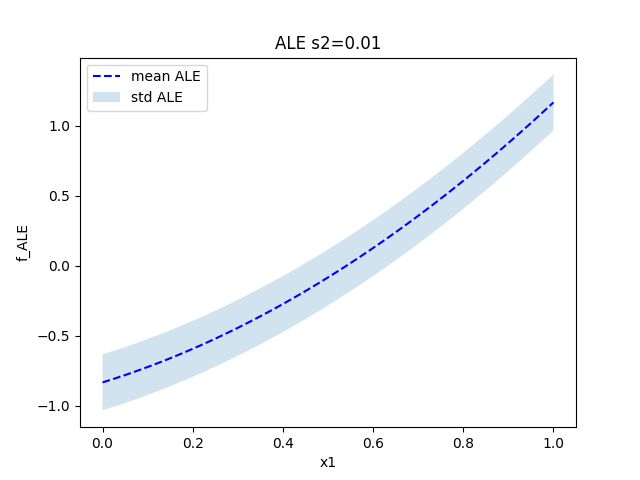
\includegraphics[width=.32\linewidth]{./example_gromping_paper/ALE_gt_s2_0_01.png}
  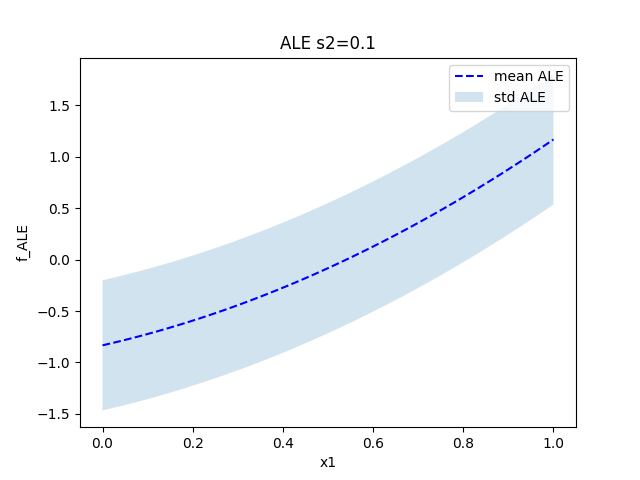
\includegraphics[width=.32\linewidth]{./example_gromping_paper/ALE_gt_s2_0_1.png}
  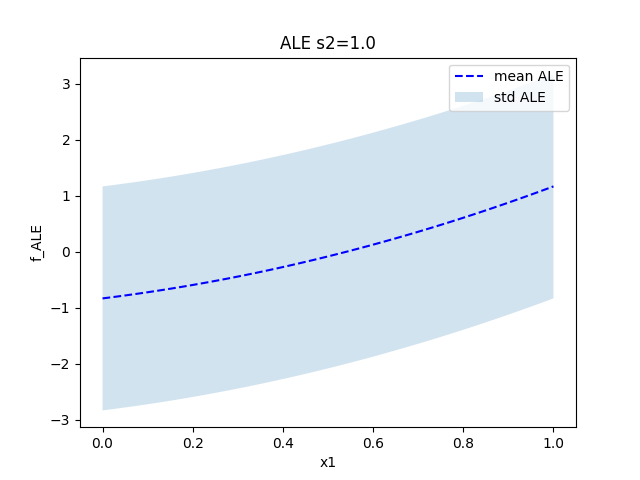
\includegraphics[width=.32\linewidth]{./example_gromping_paper/ALE_gt_s2_1_0.png}
  \caption{ALE (a) \(\sigma_2^2 = 0.01\), (b) \(\sigma_2^2 = 0.1\), (c) \(\sigma_2^2 = 1.\)}
  \label{fig:bullet-1-im-3}
\end{figure}


\paragraph{Bin Splitting.}

In figure~\ref{fig:im2}, set up for
\(b_0=0, b_1=1, b_2=1, b_3=2, \sigma_2^2 = 0.1\). Therefore, the
unavoidable uncertainty is \(\sigma^2(x_1) = b_3^2 \sigma_2^2 =
0.4\). We observe that as the bins become more dense the added
uncertainty due to binning becomes less. But as the bins become more
dense, less points lie inside them and the estimation is poor. The
vertical lines show the maximum number of bins for dataset sizes, if I
want at least 25 points per bin.


\begin{figure}[!h]
  \centering
  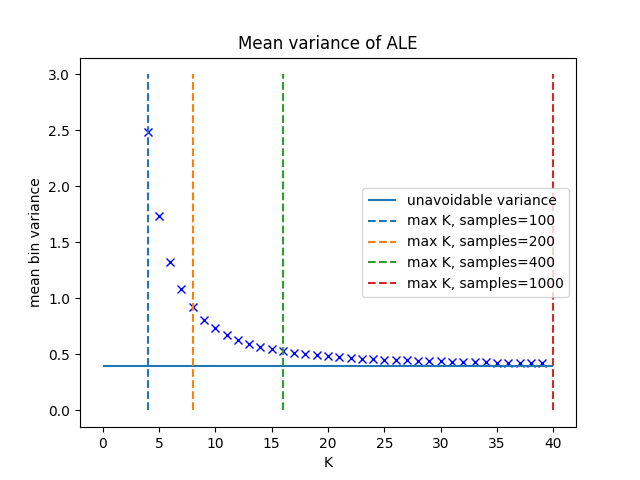
\includegraphics[width=.7\linewidth]{./example_gromping_paper/bin_varinace.png}
  \caption{}
  \label{fig:im2}
\end{figure}


\section{Evaluation}

\paragraph{Experiments.}

% Design two artificial examples to convince
% that:

% \begin{itemize}
% \item It is important to quantify the uncertainty of the explanation
%   \(\Rightarrow\) Design an example where we can obtain the
%   ground-truth ALE effect and show the change in the uncertainty as we
%   subsample the training set. Show qualitatively that the variance
%   (and the standard error) is growing as we subsample the training
%   set. Show that variance and standard error are valid compared to the
%   ground truth.
% \item It is important to split the feature axis in appropriate
%   non-overlaping bins \(\Rightarrow\) Design an example where by
%   changing the number of bins we observe that: with large bins, we
%   compute a coarse-scale ALE estimation missing fine-grain details
%   and, if ALE estimation instead of DALE, suffers from OOD
%   sampling. With small bins, the estimation of \(\mu\), \(\sigma^2\)
%   (computed only in non-empty bins and interpolated in the others) is
%   noisy. Show that with variable-size bins optimized to minimize the
%   variance we obtain the best estimation.

% \end{itemize}


\paragraph{Metrics.}

% Normalized Mean Squared Error (NMSE) between
% ground truth and approximation.


% \begin{table}[!h]
%   \centering
%   \begin{tabular}{|c|c|c|}
%     - & \texttt{ALE} vs \texttt{GT\_ALE} & ALE \\
%     \hline
%     \multirow{4}{*}{\texttt{Metric}} & \texttt{KL-Divergence} & \\
%     & \texttt{JS-Divergence} & \\
%     & \(r^2\) (\(\mu^2,\hat{\mu}^2\)) & \\
%     & \texttt{NMSE} (\(\mu^2,\hat{\mu}^2\)) & \\
%   \end{tabular}
%   \caption{Metrics that can be used}
%   \label{tab:metrics}
% \end{table}



\bibliographystyle{plain}
\bibliography{summary_bibliography.bib}

\end{document}